% capitulo7_pruebas.tex
% Capitulo 7: Resultados experimentales y analisis
%
% Autor: Leon Elliott Fuller
% Fecha: Mayo 2026

\chapter{Resultados experimentales y análisis}
\label{ch:resultados}

\section{Introducción}
\label{sec:res-intro}

Este capítulo presenta y analiza los resultados obtenidos al ejecutar la suite de benchmarking descrita en el capítulo~\ref{ch:implementacion}. El objetivo no es solo exponer cifras de rendimiento, sino interpretarlas a la luz de los tres ejes de comparación que vertebran el trabajo: RSA frente a ECC, coordenadas afines frente a Jacobianas, y cuerpos primos $\mathbb{F}_p$ frente a cuerpos binarios $\mathbb{F}_{2^m}$.

Todas las mediciones se obtuvieron con el protocolo detallado en la sección~\ref{subsec:impl-metodologia}: tres iteraciones de calentamiento descartadas, seguidas de $N = 20$ iteraciones medidas con \texttt{std::chrono::high\_resolution\_clock} a resolución de microsegundos, empleando semilla fija (\texttt{seed} = 0) para garantizar la reproducibilidad. Salvo que se indique lo contrario, las tablas reportan la \emph{mediana} de las 20 iteraciones, por ser más robusta frente a valores atípicos que la media aritmética; la media, la desviación típica y los percentiles P5/P95 están disponibles en los ficheros CSV generados por la suite. Los tiempos se expresan en microsegundos ($\mu$s) en las tablas y, cuando favorece la legibilidad, en milisegundos (ms) en el texto.

\section{Entorno de ejecución de las mediciones}
\label{sec:res-entorno}

Las características del equipo sobre el que se ejecutaron los benchmarks se resumen en el cuadro~\ref{tab:res-hardware}. Es importante recordar que los tiempos absolutos dependen del hardware concreto; lo que resulta significativo y transferible entre máquinas son las \emph{relaciones} entre algoritmos (los \textit{speedups} y ratios), que constituyen el núcleo del análisis.

\begin{table}[htbp]
\centering
\begin{tabular}{ll}
\hline
\textbf{Componente} & \textbf{Especificación} \\
\hline
CPU              & \textit{[AMD Ryzen 9 7950X 16-Core Processor (2 threads per core)]} \\
Memoria RAM      & \textit{[64 GB DDR5]} \\
Sistema operativo & Ubuntu 24.04 (contenedor Docker) \\
Compilador       & g++ con \texttt{-std=c++17 -O2} \\
NTL / GMP        & NTL $\geq$ 11.5 sobre GMP $\geq$ 6.2 \\
Iteraciones      & 100 por benchmark (3 de calentamiento descartadas) \\
Semilla          & Fija (\texttt{seed} = 0) \\
\hline
\end{tabular}
\caption{Entorno de ejecución de las mediciones experimentales.}
\label{tab:res-hardware}
\end{table}

En total se midieron 72 benchmarks individuales, agrupados en las cuatro familias que corresponden a los modos del motor de medición: RSA (24 benchmarks), ECC sobre $\mathbb{F}_p$ en coordenadas afines (18), ECC sobre $\mathbb{F}_p$ en coordenadas Jacobianas (15) y ECC sobre $\mathbb{F}_{2^m}$ (15).

\section{Rendimiento de RSA}
\label{sec:res-rsa}

El cuadro~\ref{tab:res-rsa} recoge los tiempos de las operaciones de RSA para los cuatro tamaños de clave evaluados, junto con su nivel de seguridad equivalente según NIST SP~800-57~\cite{nist-sp800-57}.

\begin{table}[htbp]
\centering
\small
\begin{tabular}{lrrrr}
\hline
\textbf{Operación} & \textbf{1024 bits} & \textbf{2048 bits} & \textbf{3072 bits} & \textbf{4096 bits} \\
                   & \textbf{(80 b)}    & \textbf{(112 b)}   & \textbf{(128 b)}   & \textbf{(140 b)} \\
\hline
Generación de clave & 1\,913   & 12\,486  & 62\,999  & 168\,953 \\
Cifrado             & 3        & 10       & 22       & 38 \\
Descifrado directo  & 178      & 1\,240   & 3\,807   & 8\,885 \\
Descifrado CRT      & 59       & 361      & 1\,097   & 2\,499 \\
Firma               & 58       & 360      & 1\,091   & 2\,525 \\
Verificación        & 3        & 10       & 22       & 38 \\
\hline
\end{tabular}
\caption{Tiempos de RSA (mediana, en $\mu$s) por tamaño de clave.}
\label{tab:res-rsa}
\end{table}

\begin{figure}[htbp]
    \centering
    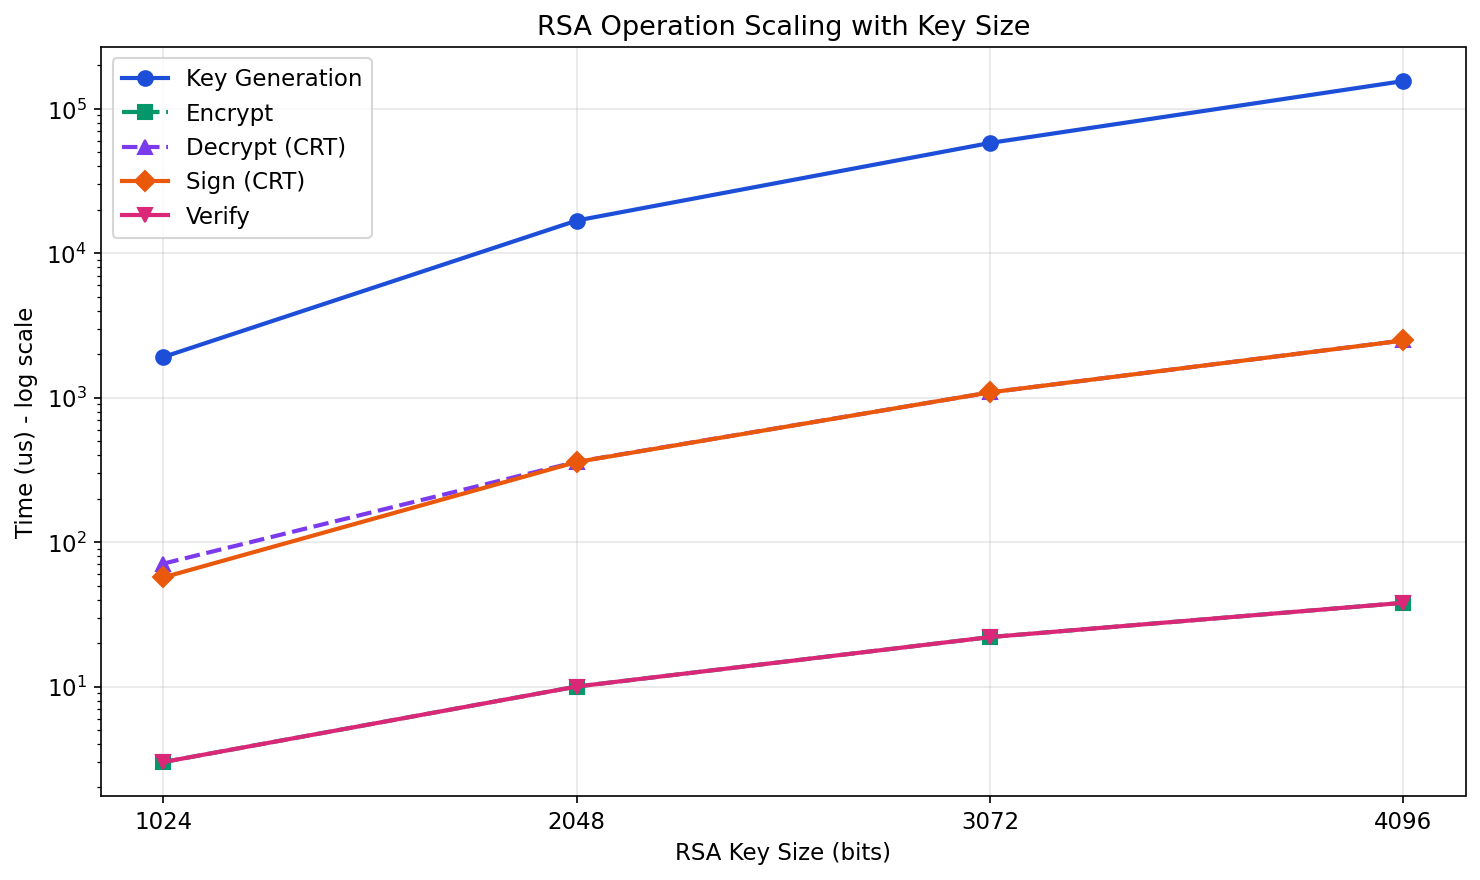
\includegraphics[width=0.85\textwidth]{imagenes/chart_rsa_scaling.png}
    \caption{Escalado de las operaciones de RSA con el tamaño de clave. Obsérvese la escala logarítmica del eje vertical: el coste de las operaciones con clave privada crece de forma marcadamente superlineal.}
    \label{fig:res-rsa-scaling}
\end{figure}

De estos datos se desprenden tres observaciones relevantes:

\paragraph{Asimetría entre operaciones públicas y privadas.}
El cifrado y la verificación son extraordinariamente rápidos (3--38~$\mu$s) y prácticamente independientes del coste de la clave privada, porque emplean el exponente público $e = 65537$, de tan solo 17~bits. En cambio, las operaciones con clave privada (descifrado, firma) usan el exponente privado $d$, del tamaño completo del módulo, y son entre uno y dos órdenes de magnitud más lentas. Esta asimetría es una característica definitoria de RSA y será determinante en la comparación con ECC.

\paragraph{Eficacia del Teorema Chino del Resto.}
El descifrado con la optimización CRT es consistentemente unas $3{,}5$ veces más rápido que el descifrado directo (por ejemplo, $1\,097$~$\mu$s frente a $3\,807$~$\mu$s a 3072~bits). Esto concuerda con la teoría: el CRT reemplaza una exponenciación módulo $n$ por dos exponenciaciones módulo $p$ y $q$, cada una con operandos de la mitad de tamaño, y el coste de la exponenciación modular crece de forma aproximadamente cúbica con el número de bits.

\paragraph{Crecimiento superlineal y varianza de la generación de claves.}
La generación de claves es la operación más costosa con diferencia, y crece de forma drástica: pasar de 1024 a 4096~bits multiplica el tiempo por un factor cercano a 90. Además, es la operación con mayor varianza: para 4096~bits, la mediana es de $168\,953$~$\mu$s ($\approx$169~ms) pero la media asciende a $223\,378$~$\mu$s ($\approx$223~ms), con un mínimo de 27~ms y un máximo de 508~ms. Esta enorme dispersión (desviación típica de $\approx$143~ms) se debe a la naturaleza probabilística de la generación de primos: el algoritmo genera candidatos aleatorios y los somete al test de Miller-Rabin hasta encontrar dos primos probables, y el número de candidatos rechazados antes de un éxito varía considerablemente entre ejecuciones. La diferencia entre media y mediana (un factor de $1{,}32$) confirma que la distribución está sesgada hacia la derecha.

\section{Rendimiento de ECC sobre cuerpos primos}
\label{sec:res-ecc-primo}

El cuadro~\ref{tab:res-ecc-afin} presenta los tiempos de ECC en coordenadas afines para las tres curvas sobre cuerpos primos implementadas.

\begin{table}[htbp]
\centering
\small
\begin{tabular}{lrrr}
\hline
\textbf{Operación} & \textbf{secp256k1} & \textbf{P-256} & \textbf{P-384} \\
                   & \textbf{(128 b)}   & \textbf{(128 b)} & \textbf{(192 b)} \\
\hline
Generación de clave    & 728   & 775   & 1\,568 \\
Multiplicación escalar & 725   & 770   & 1\,572 \\
ECDH                   & 735   & 767   & 1\,547 \\
Firma ECDSA            & 725   & 794   & 1\,586 \\
Verificación ECDSA     & 1\,465 & 1\,565 & 3\,061 \\
\hline
\end{tabular}
\caption{Tiempos de ECC en coordenadas afines (mediana, en $\mu$s).}
\label{tab:res-ecc-afin}
\end{table}

\begin{figure}[htbp]
    \centering
    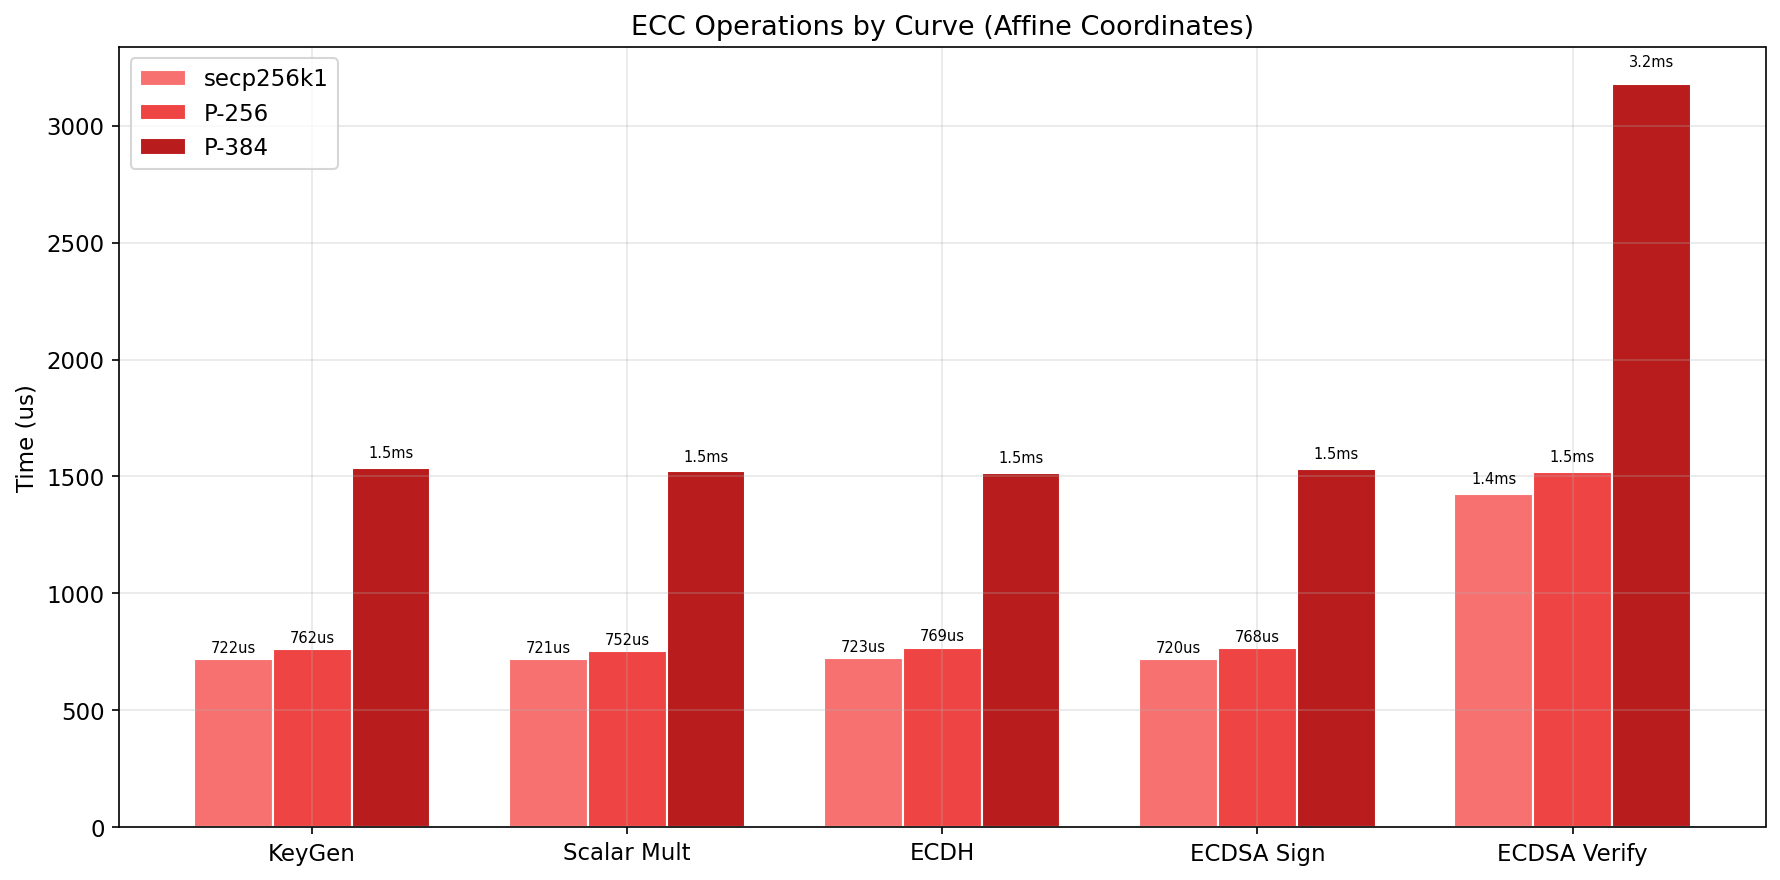
\includegraphics[width=0.85\textwidth]{imagenes/chart_ecc_curves.png}
    \caption{Comparativa de operaciones entre las curvas sobre cuerpos primos.}
    \label{fig:res-ecc-curves}
\end{figure}

Los resultados confirman varias predicciones teóricas:

\paragraph{La multiplicación escalar domina el coste.}
La generación de clave, la multiplicación escalar, el ECDH y la firma tienen tiempos casi idénticos dentro de cada curva (en torno a 725~$\mu$s para secp256k1). Esto es esperable, ya que las cuatro operaciones consisten esencialmente en una única multiplicación escalar $k \cdot P$, que es la operación computacionalmente dominante en ECC (sección~\ref{subsec:ecc-mult-escalar}).

\paragraph{La verificación cuesta el doble.}
La verificación ECDSA es aproximadamente $2{,}0$ veces más lenta que la firma (por ejemplo, $1\,465$~$\mu$s frente a $725$~$\mu$s en secp256k1). El motivo es directo: verificar una firma requiere calcular $u_1 G + u_2 Q$, es decir, \emph{dos} multiplicaciones escalares, frente a la única que necesita la firma.

\paragraph{Escalado con el tamaño del cuerpo.}
P-384 (cuerpo de 384~bits) es aproximadamente $2{,}1$ veces más lenta que las curvas de 256~bits. El coste de la multiplicación escalar crece con el número de operaciones de cuerpo (proporcional al número de bits del escalar) y con el coste de cada operación de cuerpo (que crece con el tamaño del primo), lo que explica el incremento.

\paragraph{secp256k1 frente a P-256.}
La curva secp256k1, con $a = 0$, resulta ligeramente más rápida que P-256, con $a = -3$. La ausencia del término en $a$ en las fórmulas de grupo ahorra algunas operaciones de cuerpo por cada suma o duplicación.

\section{Eje 2: coordenadas afines frente a Jacobianas}
\label{sec:res-coordenadas}

El segundo eje de comparación mide el impacto de sustituir las coordenadas afines por las Jacobianas, cuya principal ventaja es eliminar la costosa inversión modular en cada operación de grupo, difiriéndola a una única inversión al final de la multiplicación escalar (sección~\ref{subsec:ecc-afines-jacobianas}). El cuadro~\ref{tab:res-jacobian} compara ambas representaciones.

\begin{table}[htbp]
\centering
\small
\begin{tabular}{llrrr}
\hline
\textbf{Curva} & \textbf{Operación} & \textbf{Afín} & \textbf{Jacobiana} & \textbf{Speedup} \\
\hline
secp256k1 & Multiplicación escalar & 725    & 421    & $1{,}72\times$ \\
secp256k1 & Firma ECDSA            & 725    & 417    & $1{,}74\times$ \\
secp256k1 & Verificación ECDSA     & 1\,465 & 838    & $1{,}75\times$ \\
\hline
P-256     & Multiplicación escalar & 770    & 436    & $1{,}77\times$ \\
P-256     & Verificación ECDSA     & 1\,565 & 892    & $1{,}75\times$ \\
\hline
P-384     & Multiplicación escalar & 1\,572 & 836    & $1{,}88\times$ \\
P-384     & Verificación ECDSA     & 3\,061 & 1\,625 & $1{,}88\times$ \\
\hline
\end{tabular}
\caption{Comparativa de coordenadas afines frente a Jacobianas (mediana, en $\mu$s).}
\label{tab:res-jacobian}
\end{table}

\begin{figure}[htbp]
    \centering
    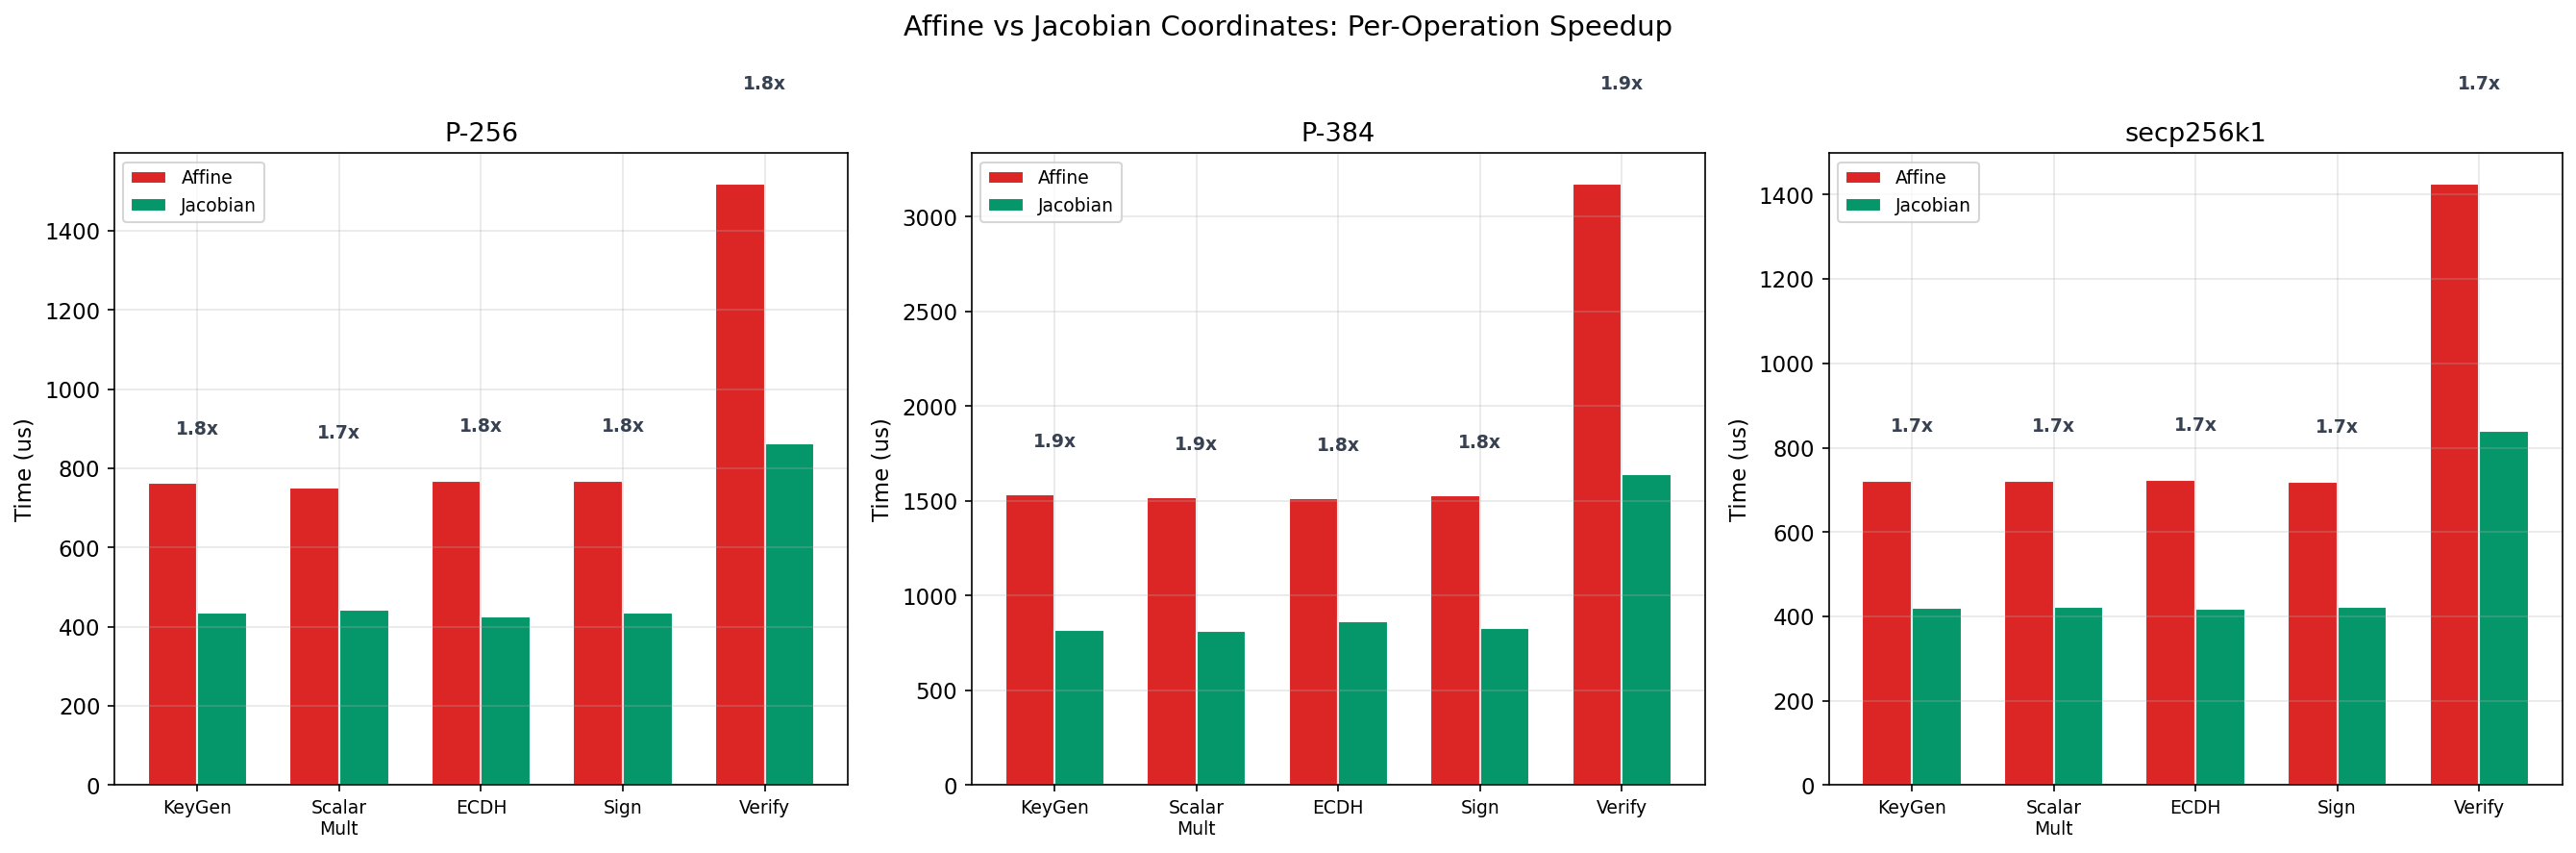
\includegraphics[width=0.85\textwidth]{imagenes/chart_affine_vs_jacobian.png}
    \caption{Comparativa de rendimiento entre coordenadas afines y Jacobianas.}
    \label{fig:res-affine-jacobian}
\end{figure}

El uso de coordenadas Jacobianas proporciona una aceleración consistente de entre $1{,}72\times$ y $1{,}93\times$ según la operación y la curva. Además, el \textit{speedup} \emph{crece} con el tamaño del cuerpo: es de $\approx 1{,}74\times$ en las curvas de 256~bits y alcanza $\approx 1{,}90\times$ en P-384. Esto es coherente con la teoría, pues la inversión modular se encarece respecto a la multiplicación a medida que aumenta el tamaño del cuerpo, de modo que eliminar inversiones reporta mayor beneficio relativo en cuerpos grandes. La figura~\ref{fig:res-jacobian-speedup} ilustra esta tendencia.

\begin{figure}[htbp]
    \centering
    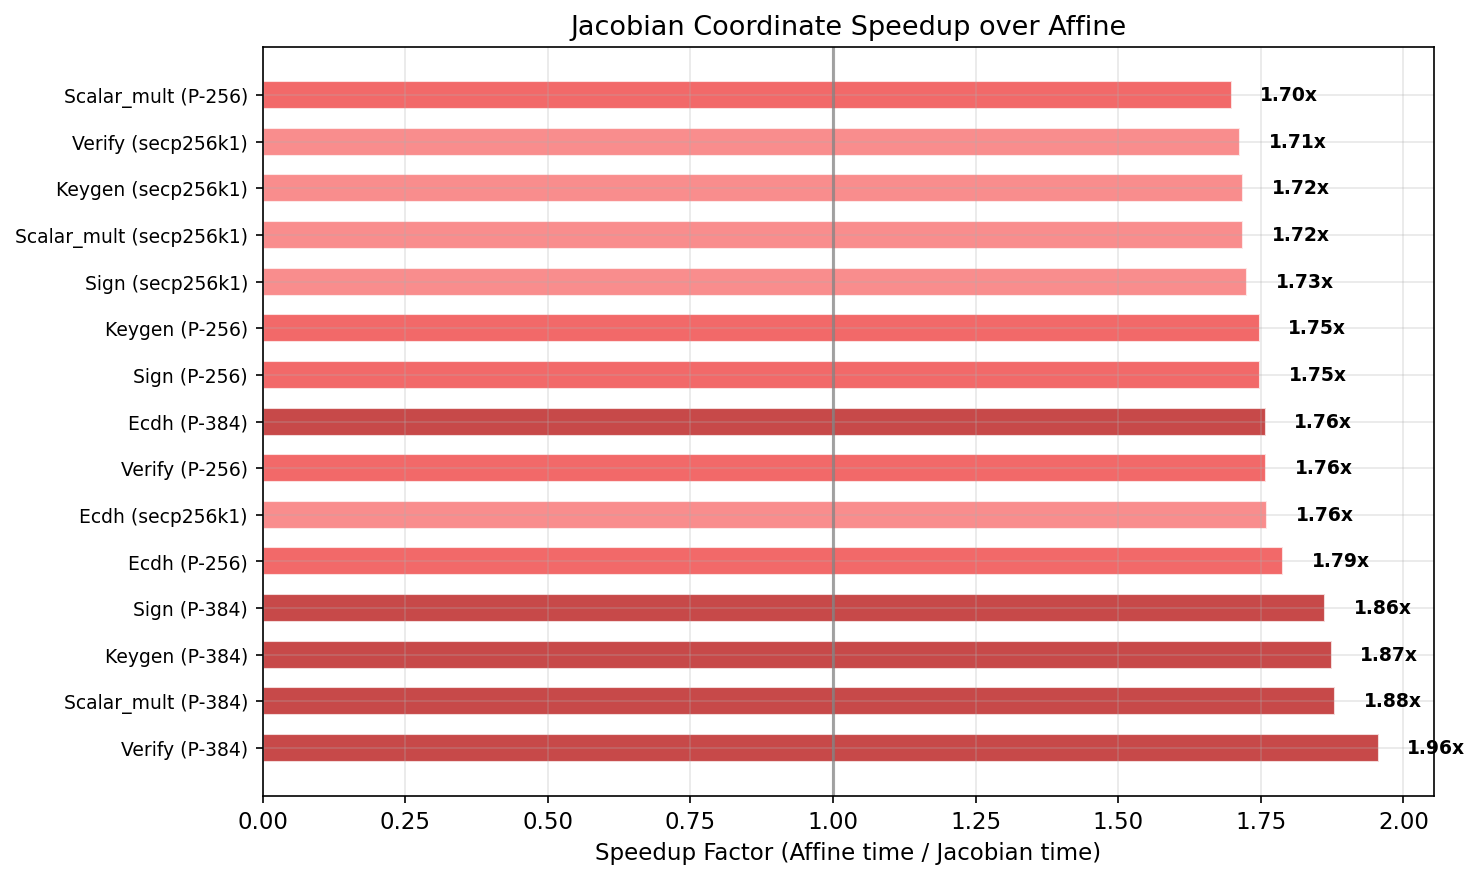
\includegraphics[width=0.8\textwidth]{imagenes/chart_jacobian_speedup.png}
    \caption{Factor de aceleración de las coordenadas Jacobianas frente a las afines, por curva.}
    \label{fig:res-jacobian-speedup}
\end{figure}

\paragraph{Interpretación del speedup observado.}
El \textit{speedup} medido ($\approx 1{,}8\times$) es real y consistente, pero más modesto que la estimación teórica basada únicamente en el conteo de operaciones, según la cual eliminar una inversión por cada operación de grupo podría sugerir aceleraciones mayores. La explicación reside en que la inversión modular de NTL, construida sobre GMP, está muy optimizada y su coste relativo frente a la multiplicación es menor que el supuesto en los modelos simplificados (que suelen asumir una inversión equivalente a 80--100 multiplicaciones). Cuando la inversión real cuesta bastante menos que ese límite, el ahorro neto de las coordenadas Jacobianas se reduce proporcionalmente. Este resultado es, de hecho, uno de los hallazgos experimentales más interesantes del trabajo: ilustra cómo las características concretas de la biblioteca aritmética subyacente pueden alterar de forma sustancial las predicciones de los modelos puramente teóricos.

\section{Eje 3: cuerpos primos frente a cuerpos binarios}
\label{sec:res-campos}

El tercer eje compara la aritmética sobre cuerpos primos $\mathbb{F}_p$ con la de cuerpos binarios $\mathbb{F}_{2^m}$. El cuadro~\ref{tab:res-binarias} recoge los tiempos de las cinco curvas binarias implementadas.

\begin{table}[htbp]
\centering
\small
\begin{tabular}{lrrr}
\hline
\textbf{Curva (seguridad)} & \textbf{Gen. clave} & \textbf{Mult. escalar} & \textbf{ECDH} \\
\hline
sect163k1 (80 b)  & 425    & 403    & 404 \\
sect233k1 (112 b) & 829    & 837    & 819 \\
sect233r1 (112 b) & 867    & 857    & 867 \\
sect283k1 (128 b) & 1\,305 & 1\,296 & 1\,263 \\
sect283r1 (128 b) & 1\,342 & 1\,251 & 1\,290 \\
\hline
\end{tabular}
\caption{Tiempos de ECC sobre cuerpos binarios $\mathbb{F}_{2^m}$ (mediana, en $\mu$s).}
\label{tab:res-binarias}
\end{table}

\begin{figure}[htbp]
    \centering
    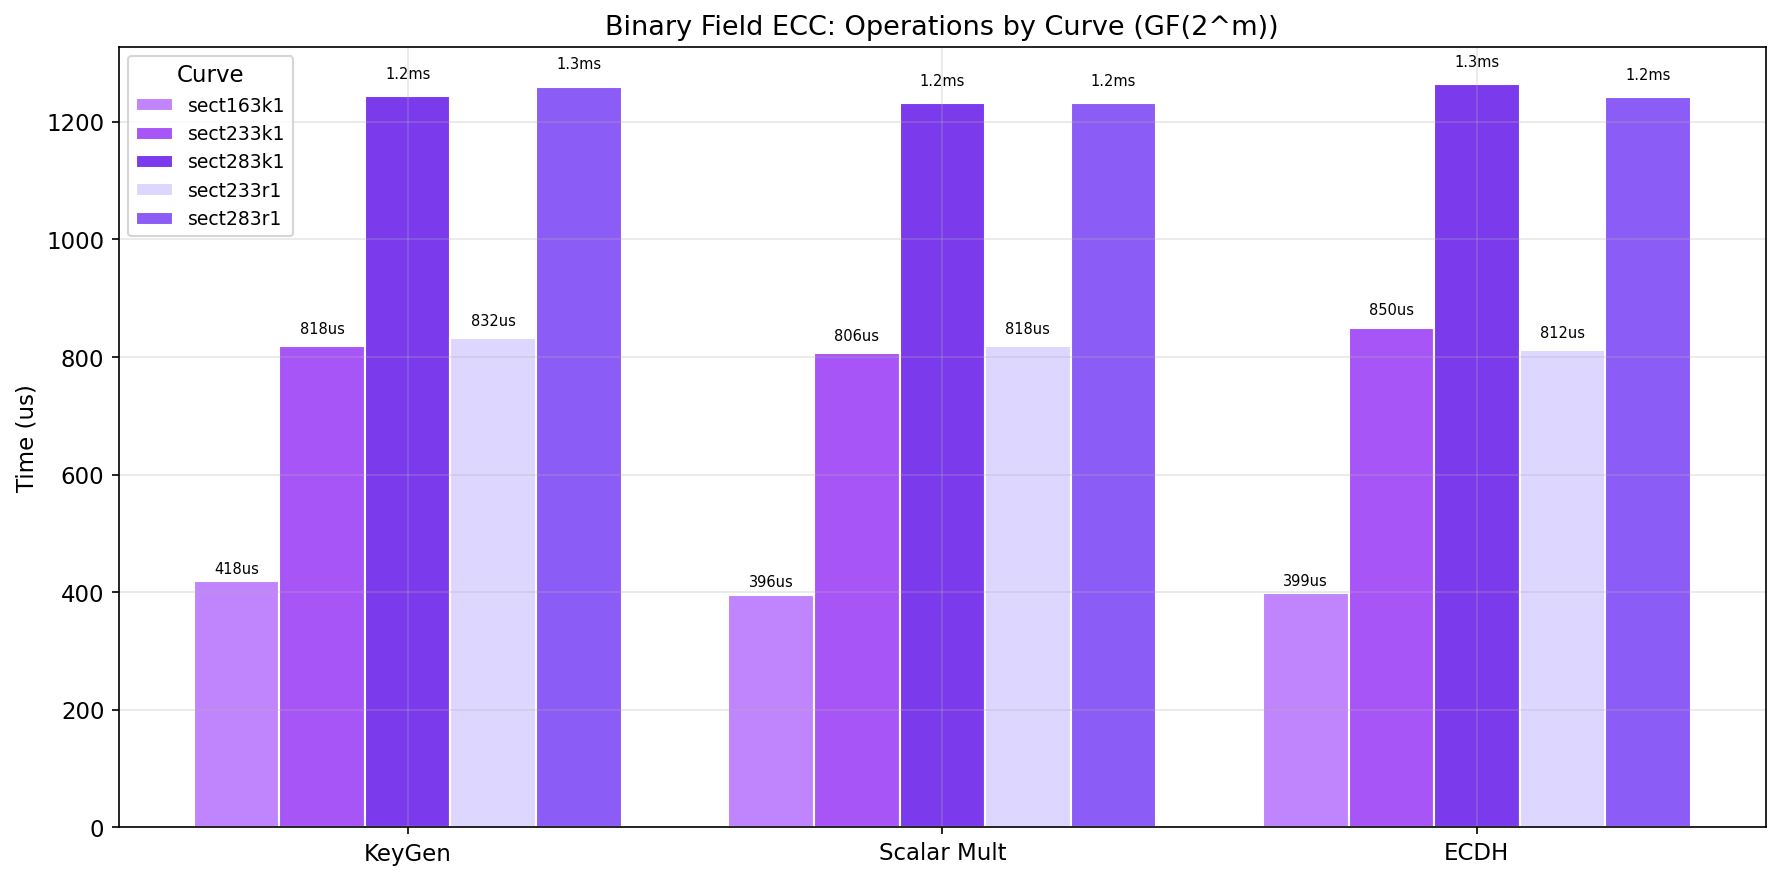
\includegraphics[width=0.85\textwidth]{imagenes/chart_binary_curves.png}
    \caption{Rendimiento de las curvas sobre cuerpos binarios.}
    \label{fig:res-binary-curves}
\end{figure}

Para comparar de forma justa ambos tipos de cuerpo, conviene situarse en un nivel de seguridad común. A 128~bits, la curva binaria sect283k1 realiza una multiplicación escalar en $1\,296$~$\mu$s, frente a los $725$~$\mu$s de la curva prima secp256k1 en coordenadas afines: la aritmética binaria resulta, por tanto, alrededor de $1{,}8$ veces más lenta. La figura~\ref{fig:res-prime-binary} visualiza esta comparación.

\begin{figure}[htbp]
    \centering
    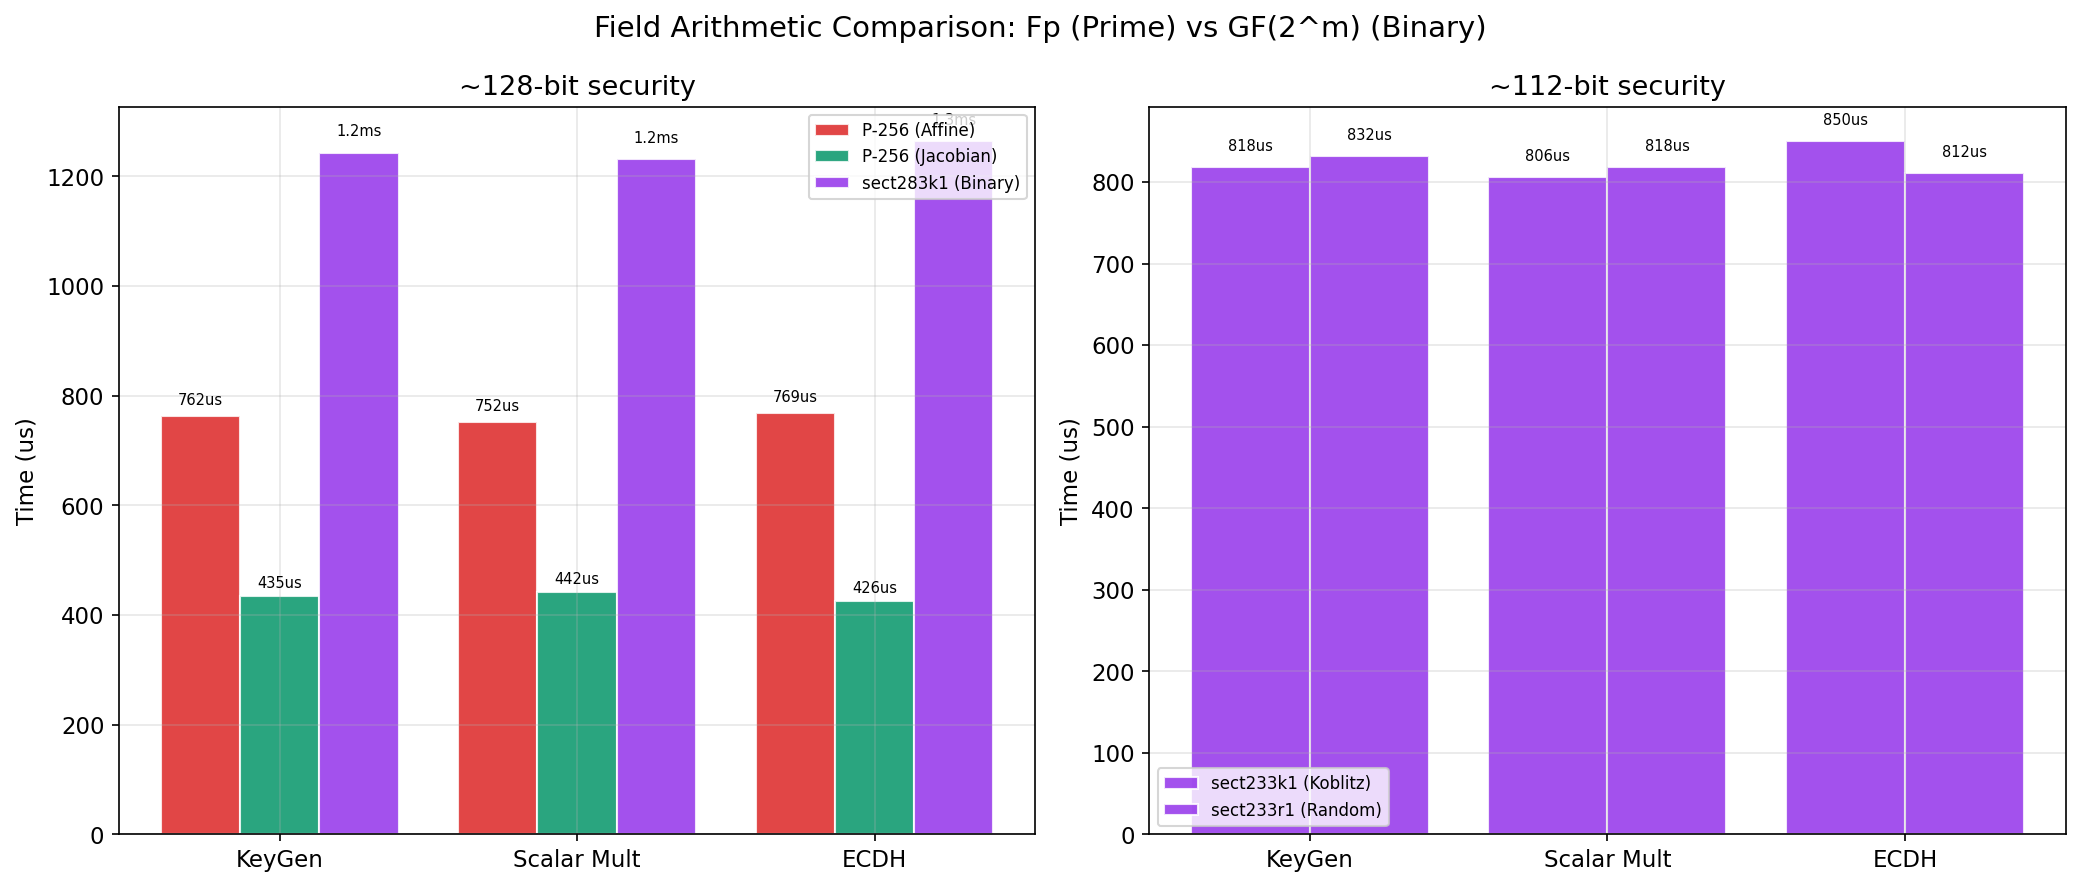
\includegraphics[width=0.85\textwidth]{imagenes/chart_prime_vs_binary.png}
    \caption{Comparativa de rendimiento entre cuerpos primos y binarios a niveles de seguridad equivalentes.}
    \label{fig:res-prime-binary}
\end{figure}

\paragraph{Un resultado dependiente de la implementación.}
Es fundamental interpretar este resultado con cautela: la desventaja de los cuerpos binarios observada aquí es un \emph{artefacto de la implementación}, no una propiedad fundamental. La aritmética sobre $\mathbb{F}_p$ se apoya en el tipo \texttt{ZZ\_p} de NTL, que delega en las rutinas de GMP optimizadas en ensamblador; en cambio, la aritmética sobre $\mathbb{F}_{2^m}$ usa \texttt{GF2E}, cuya multiplicación de polinomios no está tan finamente optimizada en este entorno de software de propósito general. En plataformas hardware (FPGA, ASIC o CPU con la instrucción de multiplicación sin acarreo \texttt{PCLMULQDQ}), la aritmética de cuerpos binarios puede igualar o superar a la de cuerpos primos, precisamente por la ausencia de propagación de acarreo. El resultado obtenido refleja, pues, el comportamiento en un entorno software puro basado en NTL, y no debe extrapolarse a contextos con soporte hardware específico.

\section{Eje 1: RSA frente a ECC a seguridad equivalente}
\label{sec:res-rsa-ecc}

El eje de comparación principal enfrenta RSA y ECC al mismo nivel de seguridad. El cuadro~\ref{tab:res-rsa-ecc} compara RSA-3072 con las curvas de 256~bits, todos ellos en el nivel de 128~bits de seguridad. Para ECC se reportan los tiempos en coordenadas Jacobianas, que representan el mejor caso de nuestra implementación.

\begin{table}[htbp]
\centering
\small
\begin{tabular}{lrrl}
\hline
\textbf{Operación} & \textbf{RSA-3072} & \textbf{ECC (secp256k1, Jac.)} & \textbf{Ventaja} \\
\hline
Generación de clave      & 62\,999 & 418 & ECC $\approx 151\times$ más rápida \\
Firma                    & 1\,091  & 417 & ECC $\approx 2{,}6\times$ más rápida \\
Operación clave privada\footnotemark & 1\,097 & 425 & ECC $\approx 2{,}6\times$ más rápida \\
Verificación             & 22      & 838 & RSA $\approx 38\times$ más rápida \\
Cifrado / operación pública & 22   & --- & RSA muy rápida ($e$ pequeño) \\
\hline
\end{tabular}
\caption{Comparativa RSA frente a ECC a 128 bits de seguridad (mediana, en $\mu$s).}
\label{tab:res-rsa-ecc}
\end{table}
\footnotetext{Descifrado CRT en RSA frente a ECDH en ECC; ambas son las operaciones representativas con material secreto.}

\begin{figure}[htbp]
    \centering
    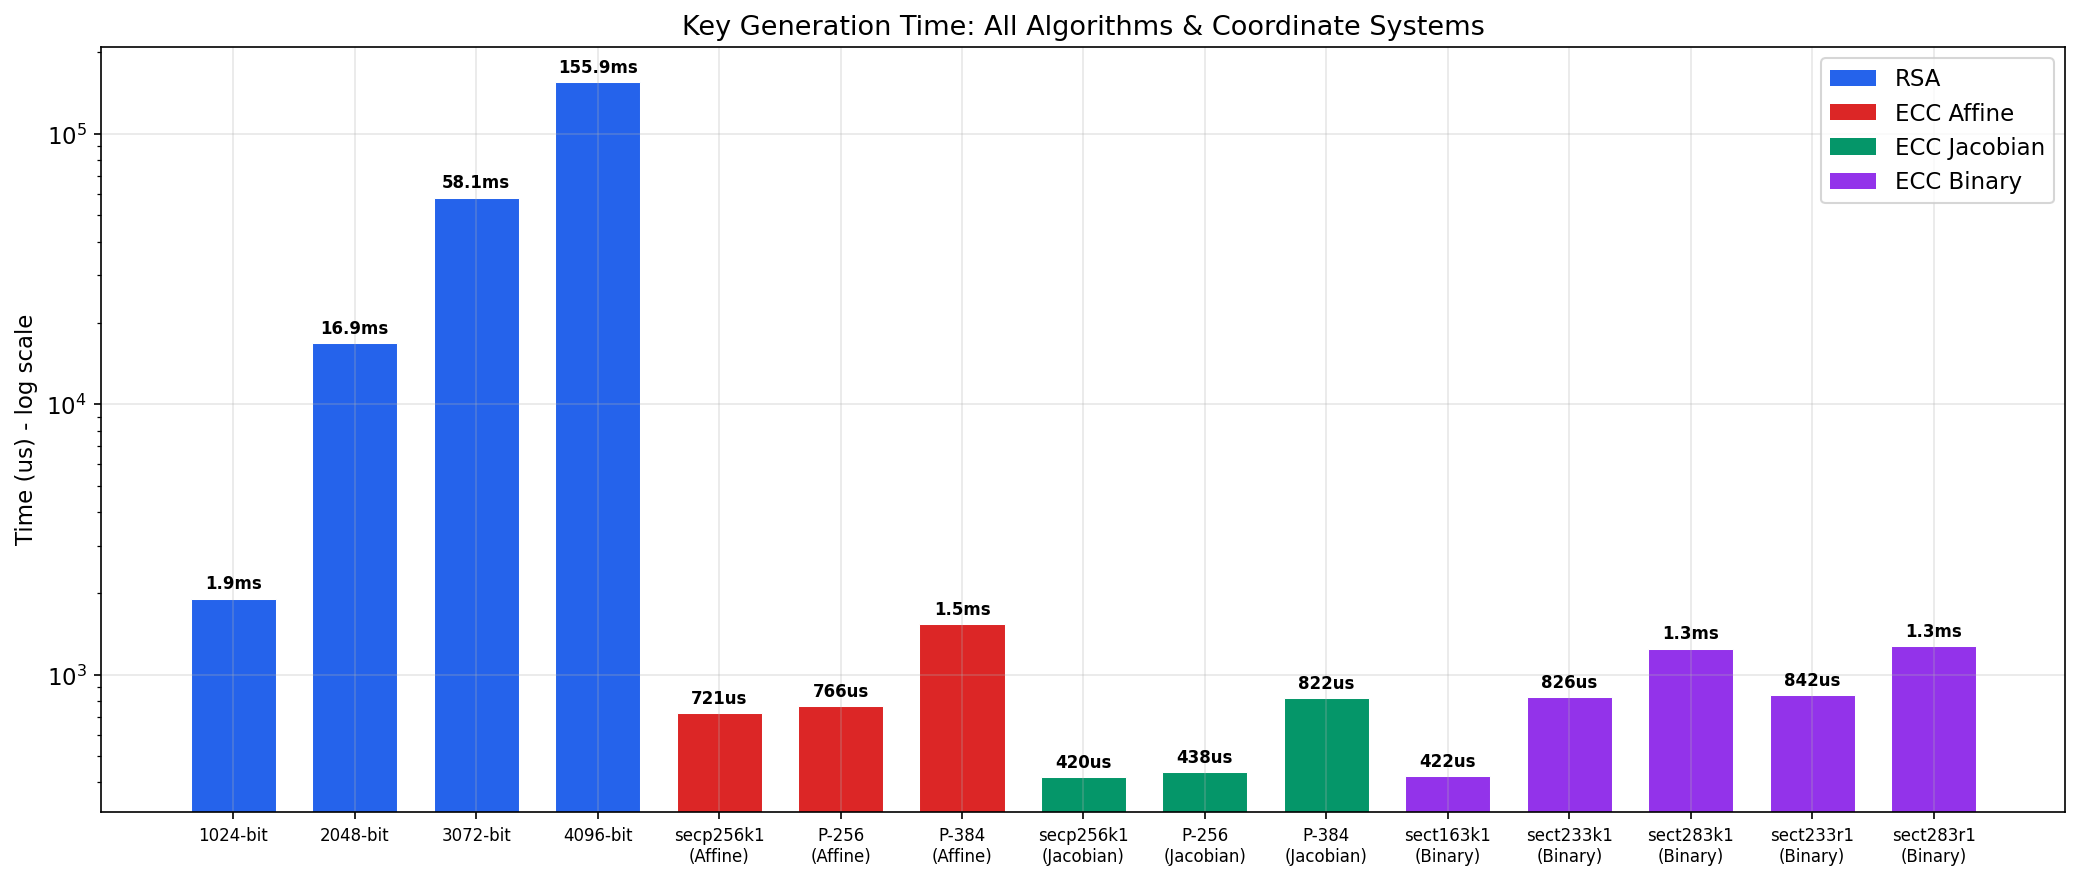
\includegraphics[width=0.85\textwidth]{imagenes/chart_keygen_comparison.png}
    \caption{Comparativa de tiempos de generación de claves entre RSA y ECC a niveles de seguridad equivalentes.}
    \label{fig:res-keygen}
\end{figure}

Este es el resultado central del trabajo, y revela una imagen matizada que desmiente la idea simplista de que ``ECC siempre es más rápida que RSA'':

\paragraph{ECC domina en generación de claves.}
La diferencia más espectacular se da en la generación de claves: ECC es unas \emph{150 veces} más rápida que RSA al mismo nivel de seguridad. Mientras RSA debe buscar dos primos grandes mediante un proceso de rechazo costoso y de varianza alta, ECC solo necesita generar un escalar aleatorio y realizar una multiplicación escalar. Para aplicaciones que generan claves con frecuencia (por ejemplo, secreto perfecto hacia adelante con claves efímeras), esta ventaja es decisiva.

\paragraph{ECC domina en firma; RSA domina en verificación.}
ECC firma $\approx 2{,}6$ veces más rápido que RSA, pero RSA verifica $\approx 38$ veces más rápido que ECC. Esta es la consecuencia directa de la asimetría de RSA: su exponente público diminuto hace que la verificación y el cifrado sean casi gratuitos, mientras que ECDSA debe realizar dos multiplicaciones escalares para verificar. La elección óptima depende, por tanto, del perfil de uso: un emisor que firma mucho (una autoridad de certificación, un servidor TLS) se beneficia de ECC, mientras que un receptor que verifica numerosas firmas (un cliente validando una cadena de certificados) puede preferir RSA.

\begin{figure}[htbp]
    \centering
    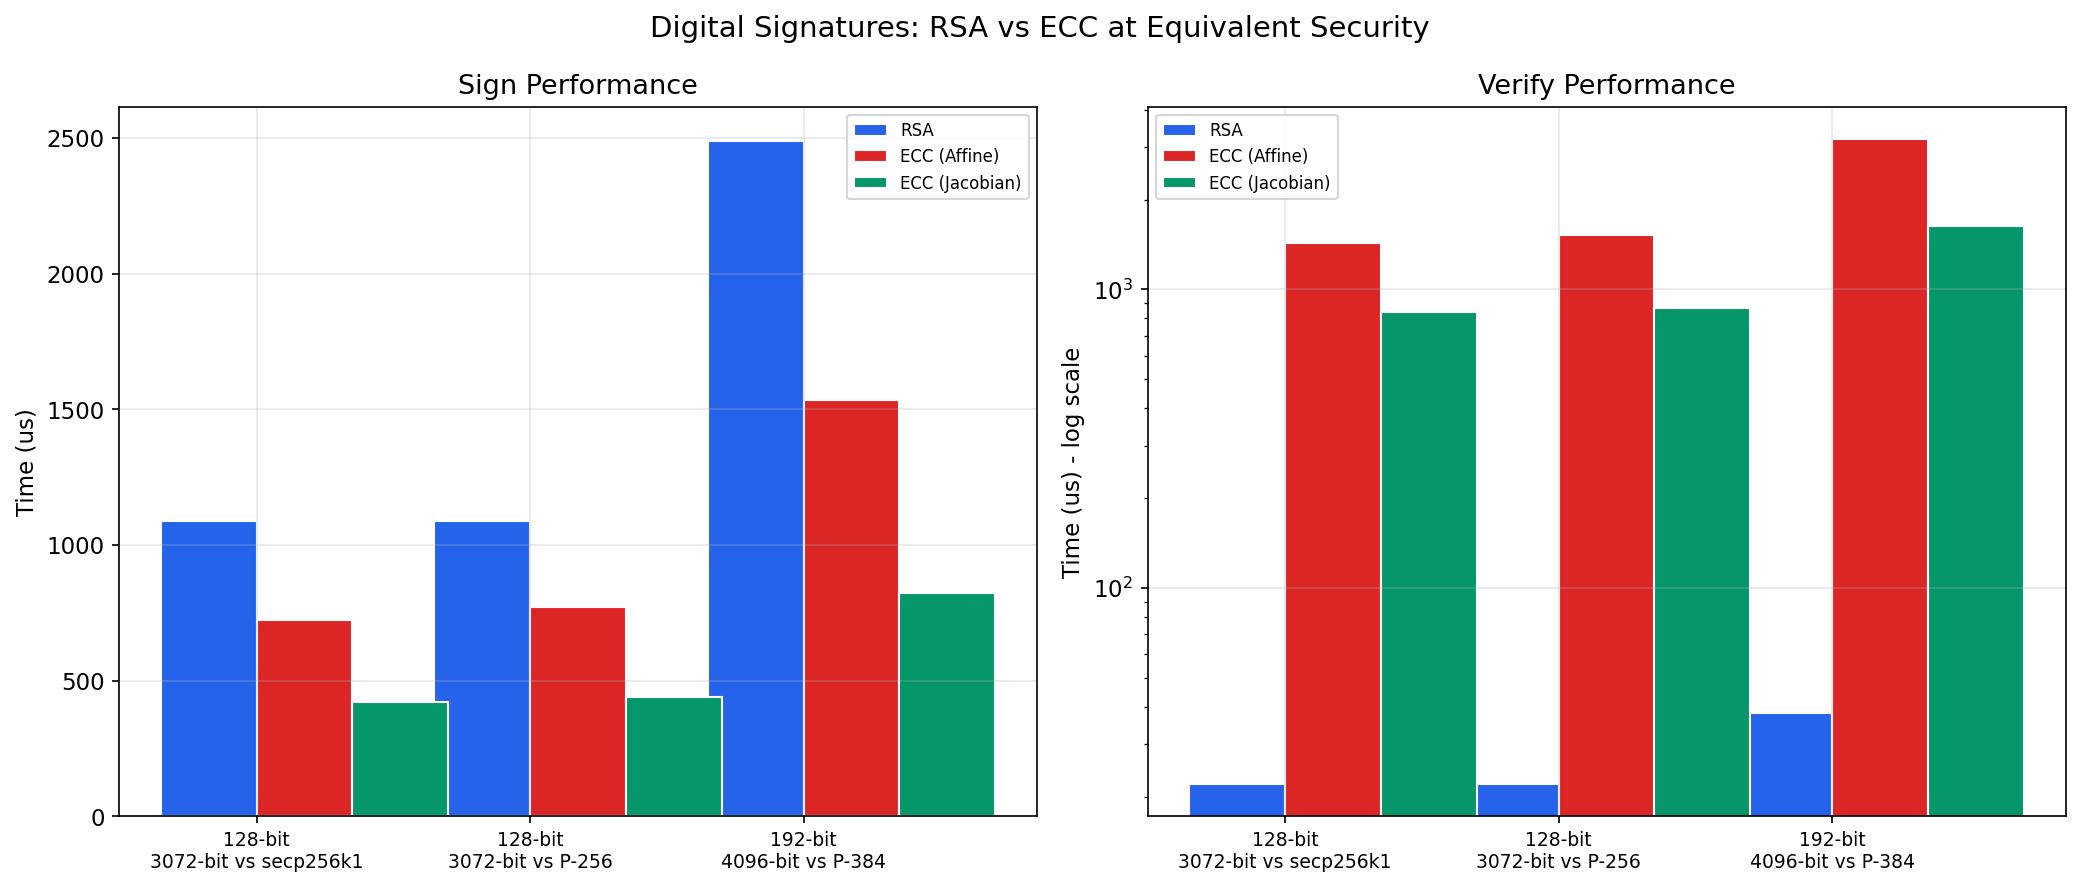
\includegraphics[width=0.85\textwidth]{imagenes/chart_sign_verify_comparison.png}
    \caption{Comparativa de las operaciones de firma y verificación entre RSA y ECC.}
    \label{fig:res-sign-verify}
\end{figure}

\paragraph{La ventaja de RSA en verificación tiene un límite.}
Aunque RSA verifica más rápido, conviene recordar que su ventaja se erosiona al aumentar el nivel de seguridad: el tamaño de clave de RSA crece mucho más deprisa que el de ECC para un mismo incremento de seguridad (3072~bits de RSA equivalen a 256~bits de curva; 7680~bits de RSA equivalen a 384~bits de curva, según se discutió en la sección~\ref{subsec:ecc-comparativa-claves}). En consecuencia, todas las operaciones de RSA, incluida la verificación, se encarecen progresivamente, mientras que las de ECC lo hacen de forma mucho más contenida. La figura~\ref{fig:res-speedup} resume los factores de aceleración entre ambos sistemas.

\begin{figure}[htbp]
    \centering
    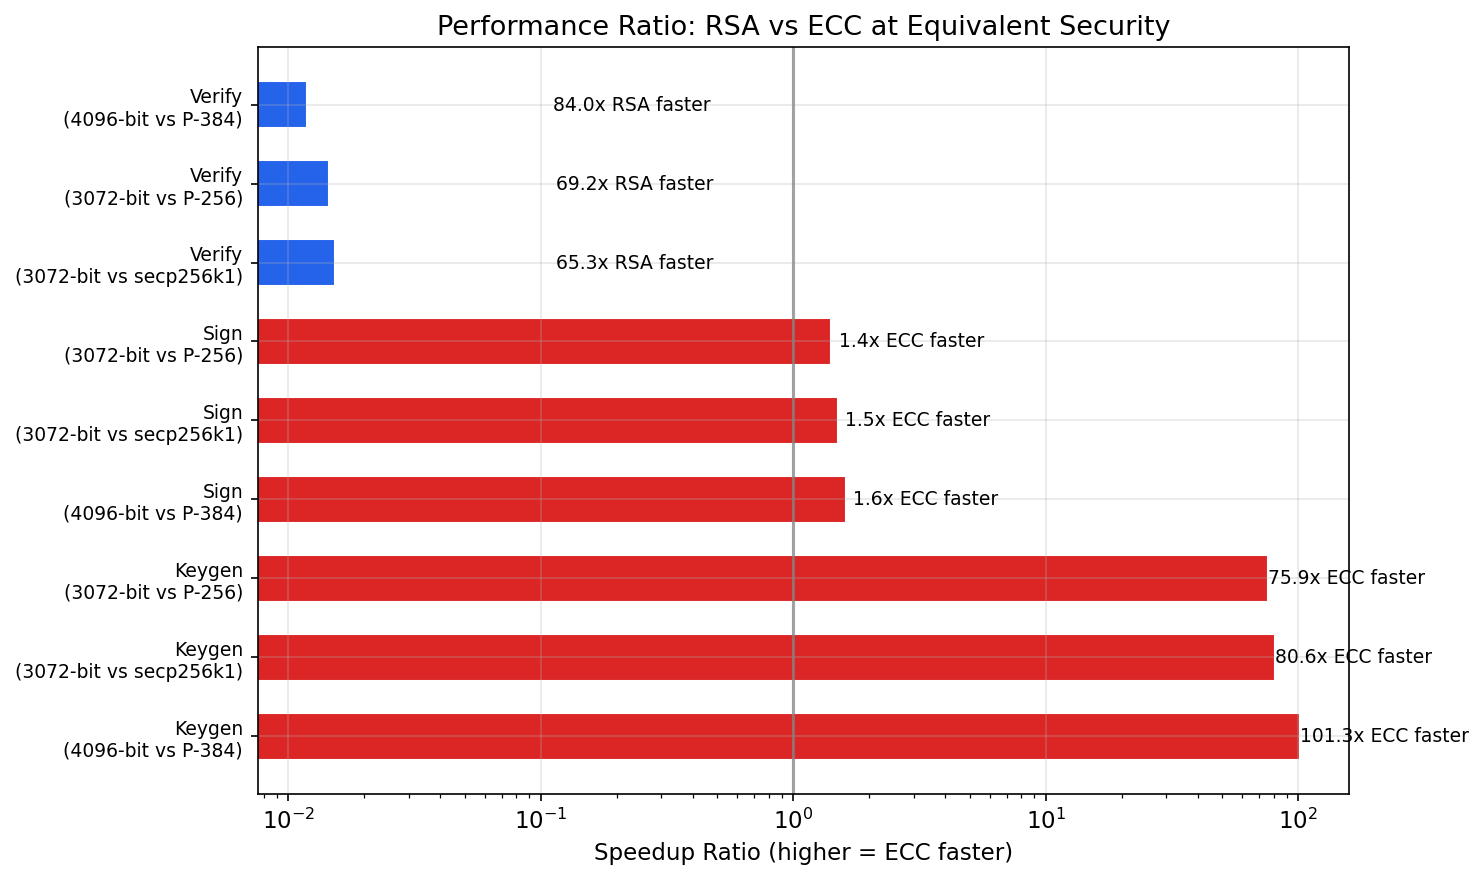
\includegraphics[width=0.85\textwidth]{imagenes/chart_speedup_ratios.png}
    \caption{Factores de aceleración relativos entre RSA y ECC por operación.}
    \label{fig:res-speedup}
\end{figure}

\paragraph{Nota sobre el nivel de 192 bits.}
La comparación a 192~bits de seguridad requeriría enfrentar RSA-7680 con P-384. Dado que la generación de una clave RSA de 7680~bits resulta prohibitivamente lenta y de varianza muy elevada, no se incluyó en la batería de pruebas; el mayor tamaño de RSA medido es 4096~bits (140~bits de seguridad). Esta limitación se asume conscientemente, pues la tendencia ya queda clara con los tamaños evaluados.

\section{Comparación con una implementación de referencia (OpenSSL)}
\label{sec:res-openssl}

Para situar los resultados en perspectiva, se compararon los tiempos de la implementación propia con los de OpenSSL~3.0.2, una biblioteca de producción ampliamente utilizada. La comparación se realizó en la misma máquina mediante la utilidad \texttt{openssl speed}. El cuadro~\ref{tab:res-openssl} recoge los resultados.

\begin{table}[htbp]
\centering
\small
\begin{tabular}{llrrl}
\hline
\textbf{Algoritmo} & \textbf{Operación} & \textbf{Propia} & \textbf{OpenSSL} & \textbf{Relación} \\
\hline
RSA-3072 & Firma        & 1\,091 & 1\,196 & Propia $1{,}10\times$ más rápida \\
RSA-3072 & Verificación & 22     & 24     & Propia $1{,}08\times$ más rápida \\
RSA-4096 & Firma        & 2\,525 & 2\,735 & Propia $1{,}08\times$ más rápida \\
RSA-4096 & Verificación & 38     & 41     & Propia $1{,}09\times$ más rápida \\
\hline
P-256 & Firma     & 440 & 13  & OpenSSL $33{,}6\times$ más rápida \\
P-256 & Verificación & 892 & 40  & OpenSSL $22{,}5\times$ más rápida \\
P-256 & ECDH      & 439 & 31  & OpenSSL $14{,}3\times$ más rápida \\
P-384 & Firma     & 829 & 521 & OpenSSL $1{,}6\times$ más rápida \\
P-384 & Verificación & 1\,625 & 411 & OpenSSL $4{,}0\times$ más rápida \\
P-384 & ECDH      & 822 & 478 & OpenSSL $1{,}7\times$ más rápida \\
\hline
\end{tabular}
\caption{Comparación de la implementación propia (ECC en coordenadas Jacobianas) con OpenSSL 3.0.2 (mediana, en $\mu$s).}
\label{tab:res-openssl}
\end{table}

Esta comparación arroja dos conclusiones de gran valor:

\paragraph{En RSA, la implementación propia es competitiva.}
Sorprendentemente, los tiempos de RSA de la implementación propia son comparables a los de OpenSSL, e incluso ligeramente mejores (en torno a un 8--10\%). La explicación es que ambas implementaciones delegan la exponenciación modular en GMP, que es donde se concentra la práctica totalidad del coste de RSA. Al compartir el mismo motor aritmético, las prestaciones convergen, y la pequeña diferencia se debe probablemente a la sobrecarga por operación que introduce el arnés de medición de OpenSSL. Este resultado valida la eficiencia de la implementación de RSA del proyecto.

\paragraph{En ECC, el margen frente a OpenSSL es grande pero revelador.}
Para ECC, OpenSSL es mucho más rápida, pero el tamaño de la diferencia es en sí mismo informativo. Para P-256, OpenSSL es entre 14 y 34 veces más rápida, porque incorpora código ensamblador escrito a mano específicamente para esta curva, la más utilizada en Internet, con aritmética de cuerpo en tiempo constante y muy optimizada. Sin embargo, para P-384 la diferencia se reduce drásticamente, a un factor de entre 1,6 y 4: al disponer OpenSSL de menos optimizaciones específicas para esta curva menos común, su implementación se acerca a una de propósito general como la nuestra. Este contraste demuestra que la brecha de rendimiento en ECC no proviene del algoritmo en sí, sino del grado de optimización a bajo nivel (ensamblador específico por curva), y que una implementación basada en NTL alcanza un rendimiento razonable en ausencia de dicho ajuste fino.

\section{Distribución estadística de las mediciones}
\label{sec:res-distribucion}

Más allá de los valores centrales, conviene examinar la distribución de las mediciones para valorar su fiabilidad. Las figuras~\ref{fig:res-dist-sign} y~\ref{fig:res-dist-verify} muestran la distribución de los tiempos de firma y verificación.

\begin{figure}[htbp]
    \centering
    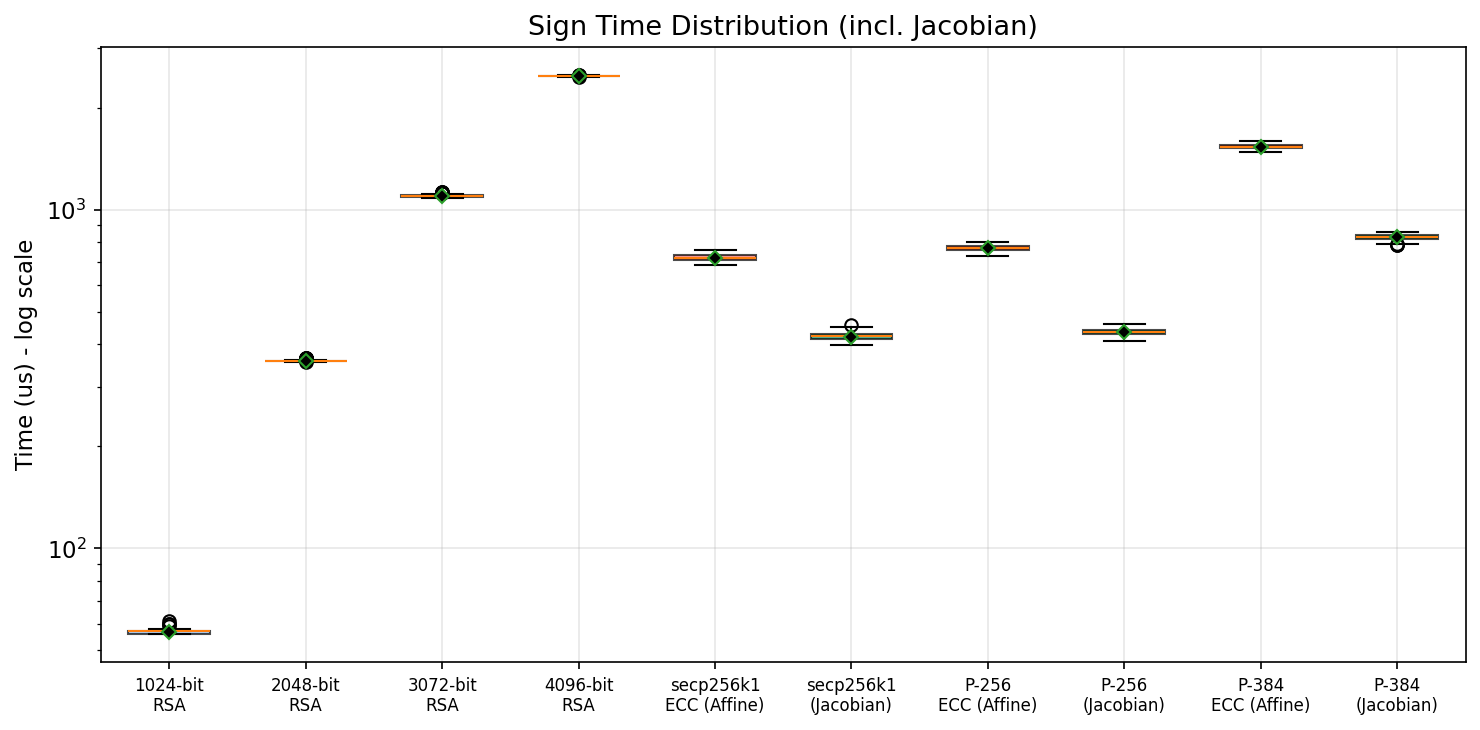
\includegraphics[width=0.85\textwidth]{imagenes/chart_distribution_sign.png}
    \caption{Distribución de los tiempos de la operación de firma.}
    \label{fig:res-dist-sign}
\end{figure}

\begin{figure}[htbp]
    \centering
    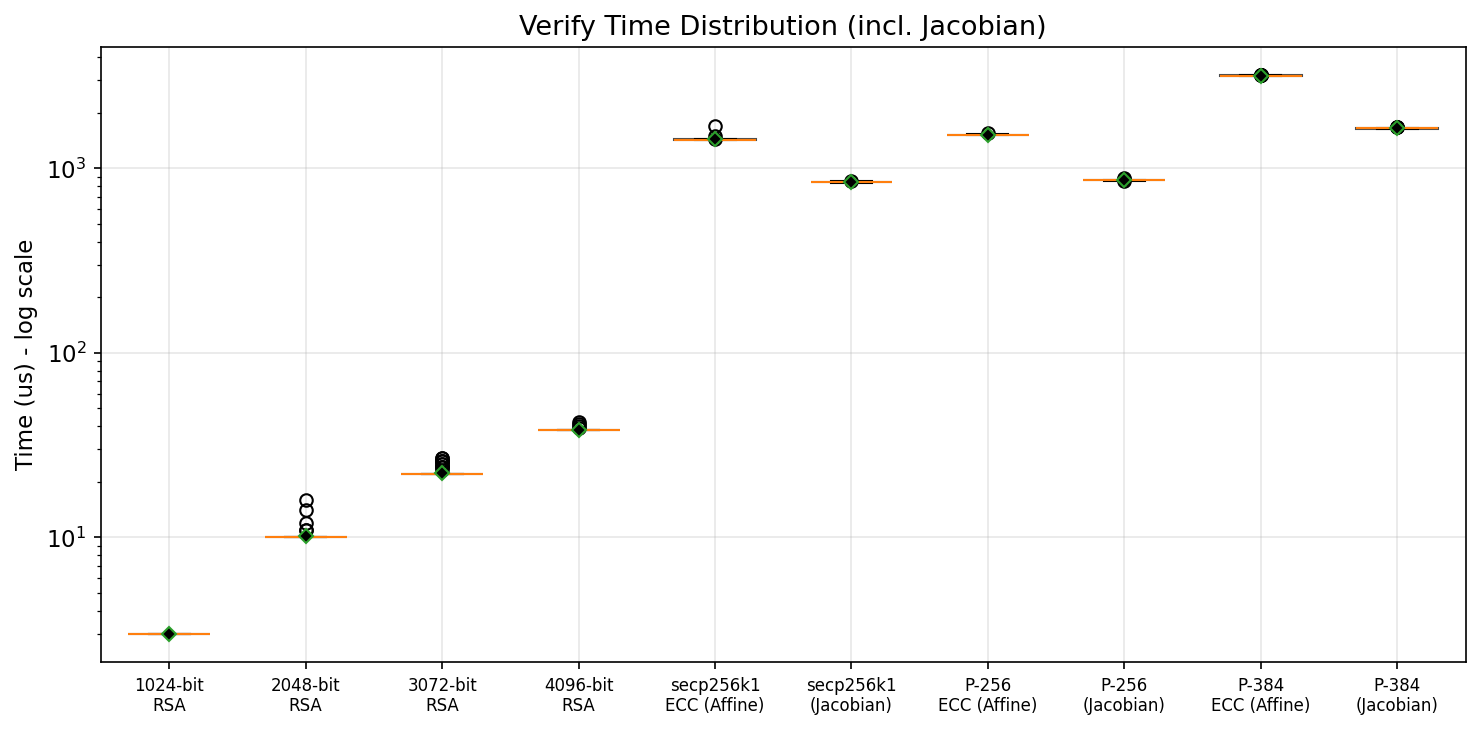
\includegraphics[width=0.85\textwidth]{imagenes/chart_distribution_verify.png}
    \caption{Distribución de los tiempos de la operación de verificación.}
    \label{fig:res-dist-verify}
\end{figure}

Para la mayoría de las operaciones de ECC y para las operaciones públicas de RSA, la desviación típica es pequeña en relación con la mediana (a menudo por debajo del 3\%), lo que indica mediciones muy estables y reproducibles, favorecidas por el uso de semilla fija y por el protocolo de calentamiento. La principal excepción, como ya se ha señalado, es la generación de claves de RSA, cuya varianza intrínseca proviene del proceso de búsqueda de primos y no de ruido en la medición.

\section{Resumen de resultados}
\label{sec:res-resumen}

La figura~\ref{fig:res-collage} ofrece una panorámica conjunta de los principales resultados, la figura~\ref{fig:res-summary-table} resume en forma de tabla los tiempos de todas las operaciones, y el cuadro~\ref{tab:res-summary} sintetiza los hallazgos a lo largo de los tres ejes de comparación.

\begin{figure}[htbp]
    \centering
    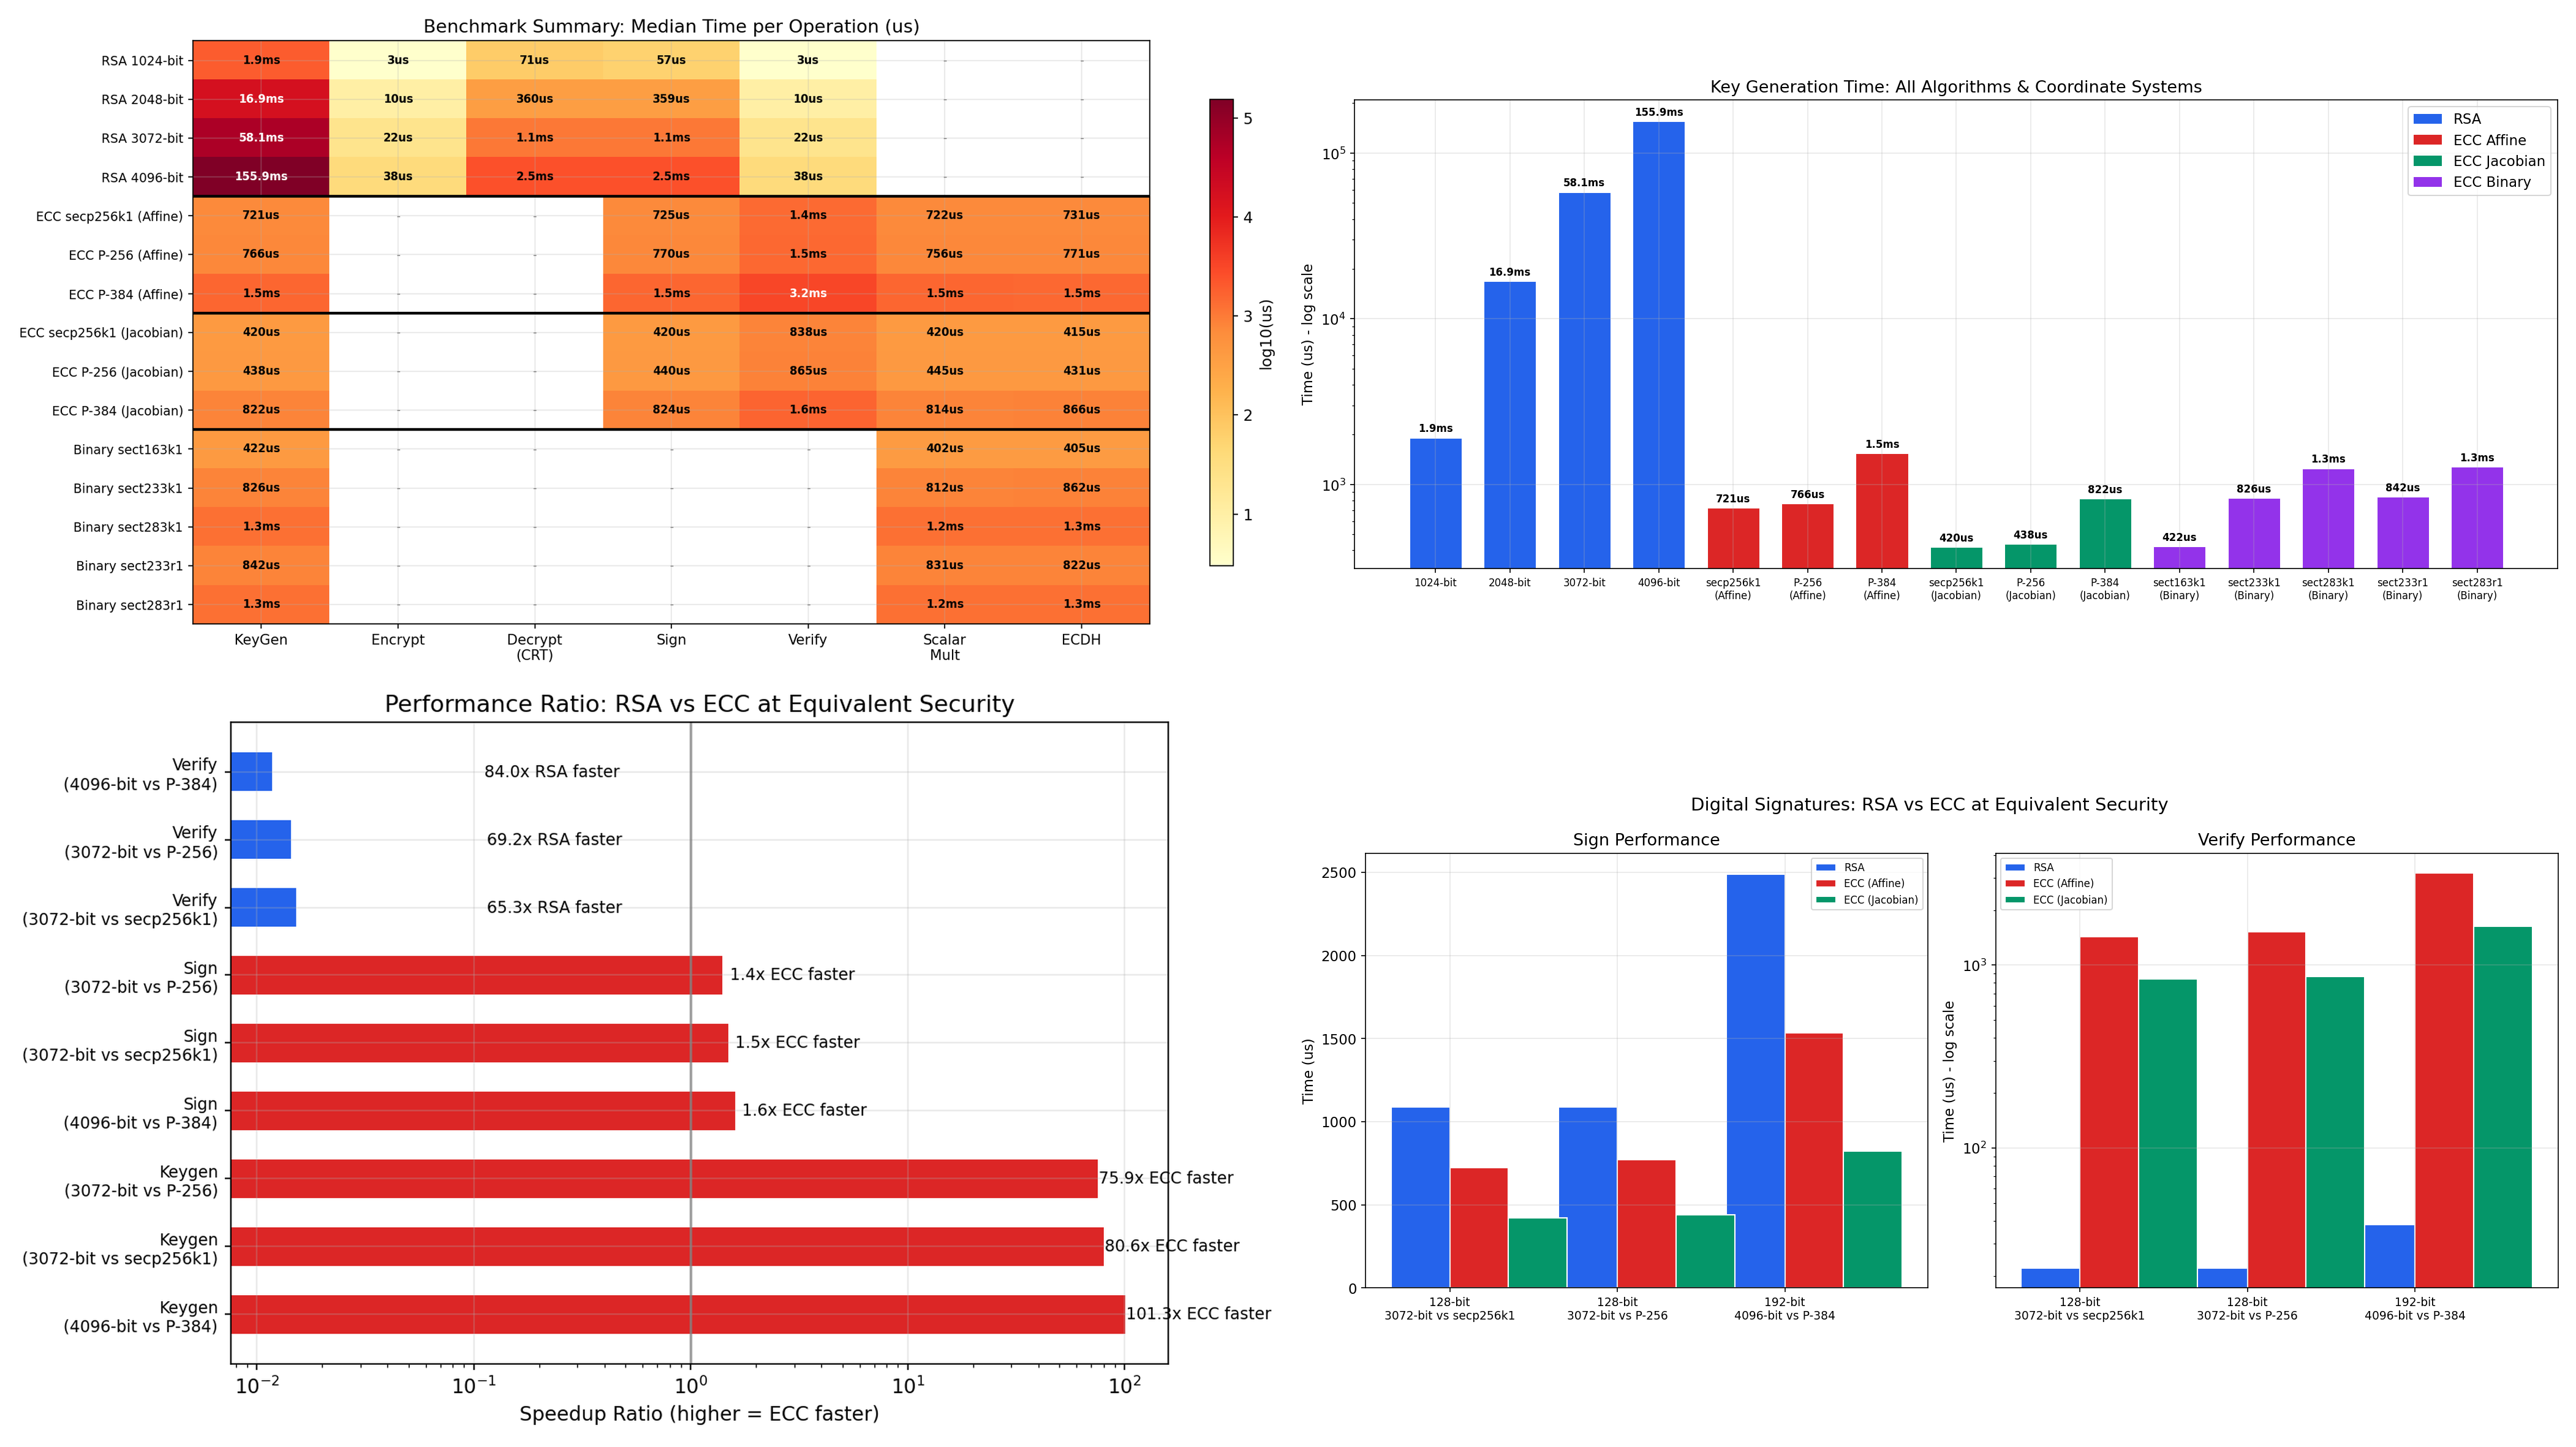
\includegraphics[width=\textwidth]{imagenes/collage_comparison.png}
    \caption{Panorámica comparativa de los resultados de rendimiento.}
    \label{fig:res-collage}
\end{figure}

\begin{figure}[htbp]
    \centering
    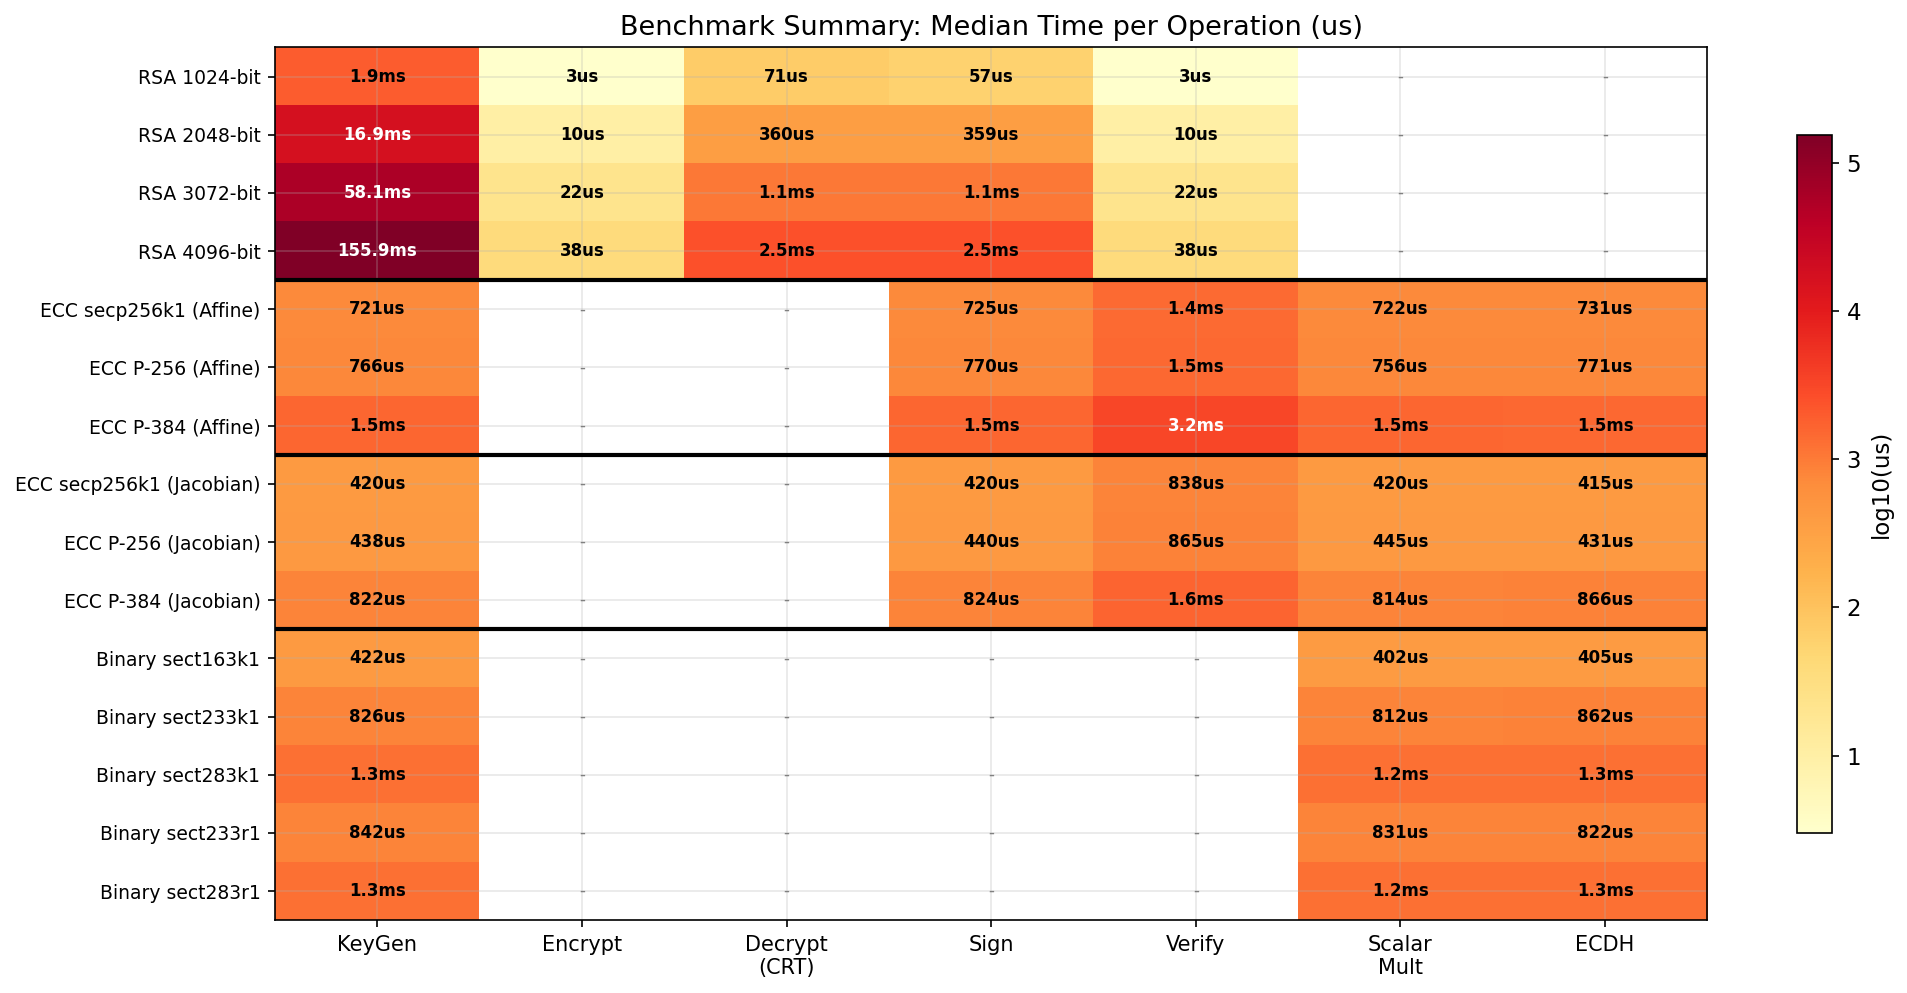
\includegraphics[width=0.9\textwidth]{imagenes/chart_summary_table.png}
    \caption{Tabla-resumen de los tiempos medidos para todas las operaciones y configuraciones.}
    \label{fig:res-summary-table}
\end{figure}

\begin{table}[htbp]
\centering
\small
\begin{tabular}{lp{9cm}}
\hline
\textbf{Eje de comparación} & \textbf{Hallazgo principal} \\
\hline
RSA frente a ECC & ECC domina con holgura en generación de claves ($\approx 150\times$) y firma ($\approx 2{,}6\times$); RSA domina en verificación ($\approx 38\times$) gracias a su exponente público pequeño. La elección óptima depende del perfil de uso. \\
\hline
Afín frente a Jacobiana & Las coordenadas Jacobianas aceleran la aritmética de curva entre $1{,}7\times$ y $1{,}9\times$, con un beneficio creciente al aumentar el tamaño del cuerpo. \\
\hline
$\mathbb{F}_p$ frente a $\mathbb{F}_{2^m}$ & En software puro con NTL, los cuerpos primos son $\approx 1{,}8\times$ más rápidos que los binarios; se trata de un artefacto de implementación, no de una propiedad fundamental. \\
\hline
Referencia OpenSSL & En RSA, la implementación propia iguala a OpenSSL (ambas usan GMP); en ECC, OpenSSL es más rápida por su ensamblador específico, con una brecha que se estrecha en curvas menos optimizadas como P-384. \\
\hline
\end{tabular}
\caption{Síntesis de los hallazgos experimentales por eje de comparación.}
\label{tab:res-summary}
\end{table}

En conjunto, los experimentos cumplen el objetivo planteado: cuantifican de forma reproducible las diferencias de rendimiento entre RSA y ECC, y caracterizan el impacto de las dos decisiones de implementación estudiadas (sistema de coordenadas y tipo de cuerpo). Las conclusiones globales que se derivan de estos resultados, junto con las líneas de trabajo futuro, se desarrollan en el capítulo~\ref{ch:conclusiones}.